\chapter{内存管理系统}

\section{系统设计}

NimlothOS的内存管理使用与xv6一样的\href{https://five-embeddev.com/riscv-priv-isa-manual/Priv-v1.12/supervisor.html#sec:sv39}{SV39}分页机制,
并实现了用户地址空间与内核地址空间分离。整体系统设计结构如下:

\begin{figure}[htbp]
    \centering
    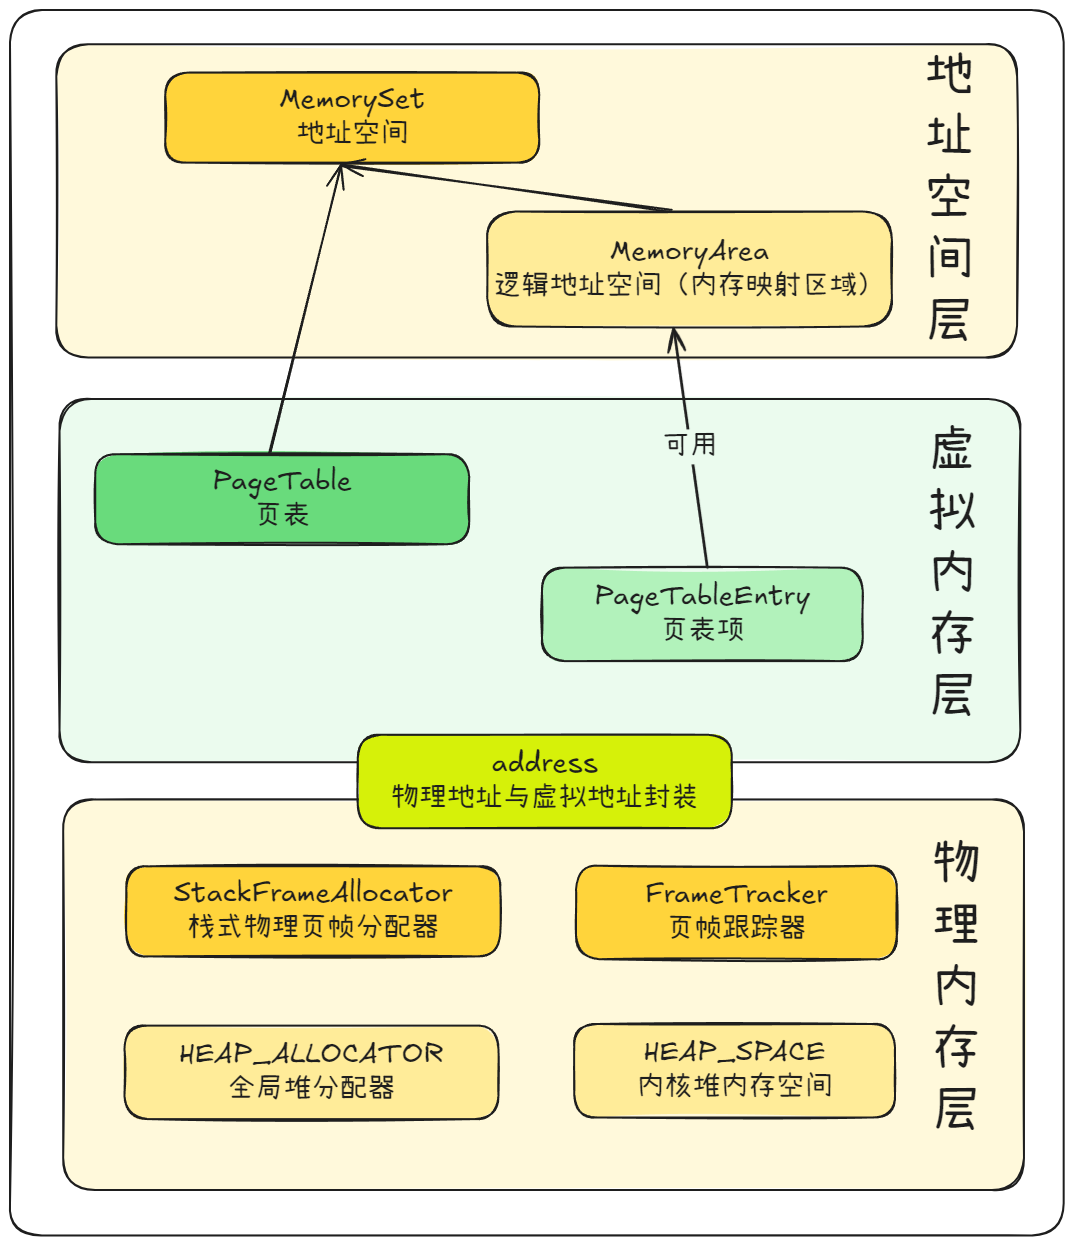
\includegraphics[width=0.4\textwidth]{../image/内存.png}
    \caption{内存系统结构}
    \label{fig:kernel-elf}
\end{figure}

\section{SV39}

Sv39的含义是它只用64bit虚拟地址的底部39位,剩下的25位不用,在这种配置中,RISC-V的页表在逻辑上是一个包含$2^{27}$个页表项的数组,每个页表项含一个44位的物理页号和一些标志位。
分页硬件通过使用39位中的顶部27位来索引页表以找到一个页表项,并生成一个56位的物理地址。物理地址的顶部44位来自页表项中的物理页号,底部12位从原始的虚拟地址中复制而来。

这里借用xv6 book中的图。

\begin{figure}[htbp]
    \centering
    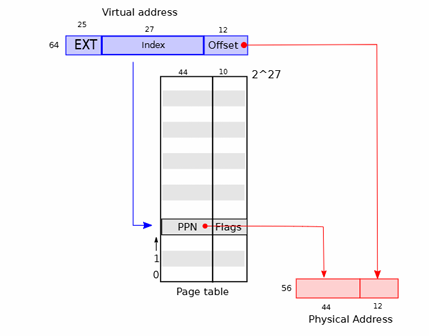
\includegraphics[width=0.4\textwidth]{../image/物理地址.png}
    \caption{物理地址}
    \label{fig:物理地址}
\end{figure}

\subsection{satp寄存器(Supervisor Address Translation and Protection Register)}

\href{https://five-embeddev.com/riscv-priv-isa-manual/Priv-v1.12/supervisor.html#sec:satp}{satp寄存器}用于控制管理模式下的地址转化与保护,其格式如下图:

\begin{figure}[htbp]
    \centering
    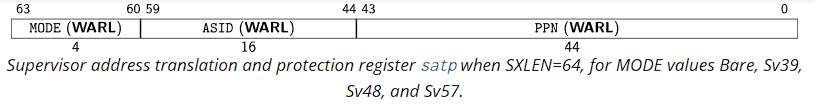
\includegraphics[width=0.8\textwidth]{../image/satp.png}
    \caption{satp寄存器}
    \label{fig:satp}
\end{figure}

当MODE没有设置时,虚拟地址即等于物理地址,当MODE设置时,就会启用分页模式,在此之后访存的地址必须
经过内存控制单元进行虚拟地址到物理地址的转换,再用它来访问物理内存。

\begin{figure}[htbp]
    \centering
    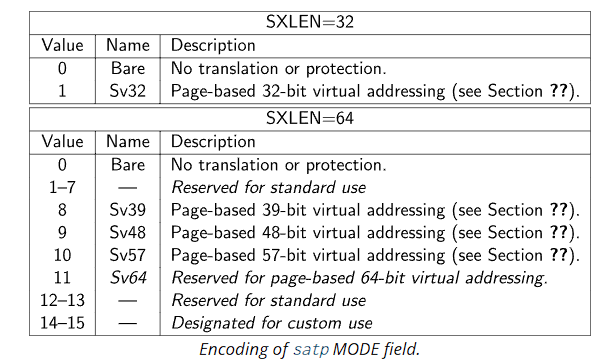
\includegraphics[width=0.6\textwidth]{../image/satpMode.png}
    \caption{satp mode字段的含义}
    \label{fig:satpMode}
\end{figure}

ASID字段用于性能优化,它可以区分不同进程的地址空间,但当前操作系统未实现,硬编码为0。如需地址空间切换时
会调用汇编命令\lstinline[language=Rust]{sfence.vma}来刷新TLB。

另外,satp寄存器的PPN处存放当前地址空间根页表的物理页号,satp的设置在内存管理系统初始化的时候完成,
此后地址空间切换也是调用汇编命令进行刷新\lstinline[language=Rust]{csrw satp, a1}。

\begin{lstlisting}[language=Rust,caption={satp设置}, label={lst:kernel-sections}]
pub fn activate(&self) {
    let satp = self.page_table.token();
    unsafe {
        satp::write(satp);
        asm!("sfence.vma");
    }
}
pub fn token(&self) -> usize {
    8usize << 60 | self.root_ppn.0
}
\end{lstlisting}

\subsection{地址格式}

\begin{figure}[htbp]
    \centering
    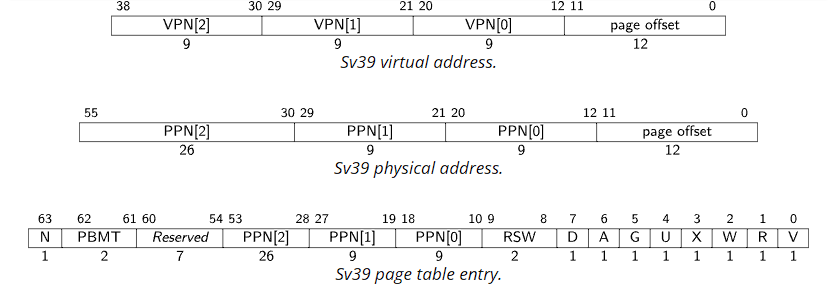
\includegraphics[width=0.8\textwidth]{../image/地址.png}
    \caption{地址与页表项}
    \label{fig:地址}
\end{figure}

虚拟地址和物理地址的低12位为页内偏移,这是因为设置单个页面大小为4KB。虚拟地址的高27位,可以看到分为L2、L1、L0,
它们是虚拟页号Virtual Page Number,物理地址的高44位同理。

页表项可以用虚拟页号为索引查到,它由物理页号和标志位组成。

值得注意的是,sv39规定\href{https://five-embeddev.com/riscv-priv-isa-manual/Priv-v1.12/supervisor.html#sec:sv39}{地址的63位到39位必须全部等于第38位},
否则将引发缺页异常。这意味着我们可以使用的地址空间只有高256G和低256G。

\subsection{地址转换}

地址转换过程中,首先会用虚拟页号的一级页索引去根页表中查二级页表的物理页号,
然后用虚拟页号的二级页索引去刚刚查到的二级页表中查三级页表的物理页号,
再用三级页索引在三级页表的物理页中查到物理页号,它与页内偏移拼接后就可得到物理地址。

\begin{figure}[htbp]
    \centering
    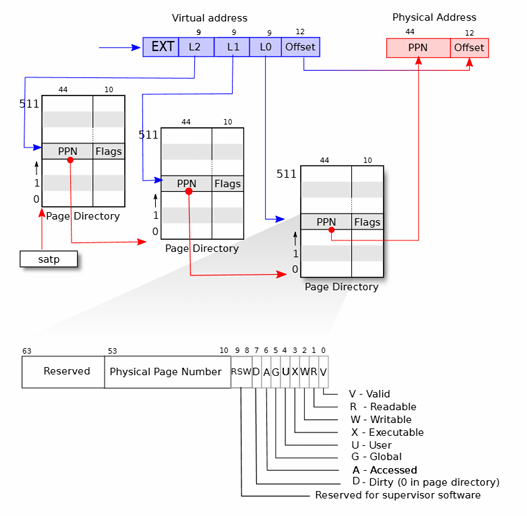
\includegraphics[width=0.7\textwidth]{../image/地址转换.png}
    \caption{地址转换}
    \label{fig:地址转换}
\end{figure}

\section{动态内存分配}

NimlothOS的内存管理包含两个层次的动态内存分配:堆分配器和物理页帧分配器。
堆分配器管理内核中的动态数据结构,而物理页帧分配器管理4KB大小的物理页面。

\subsection{堆分配器}

内存堆分配器负责管理内核中的动态数据结构,如向量、哈希表、字符串等。我用的是基于Buddy System算法实现的\lstinline[language=Rust]{buddy_system_allocator}库,
这种算法能够有效减少内存碎片,提供高效的动态内存管理。

系统预先为堆分配器保留了3MB的静态内存空间,该空间位于内核的BSS段中:

\begin{lstlisting}[language=Rust,caption={堆分配器声明}, label={lst:heap-decl}]
/// 全局堆分配器实例
#[global_allocator]
static HEAP_ALLOCATOR: LockedHeap<32> = LockedHeap::empty();

/// 内核堆内存空间(3MB)
static mut HEAP_SPACE: [u8; KERNEL_HEAP_SIZE] = [0; KERNEL_HEAP_SIZE];
\end{lstlisting}

\lstinline[language=Rust]{HEAP_ALLOCATOR}使用\lstinline[language=Rust]{#[global_allocator]}属性标记,使其成为Rust运行时使用的默认内存分配器。\lstinline[language=Rust]{LockedHeap<32>}中的32表示支持的最大分配块大小为$2^{32}$字节。

堆分配器的初始化过程相对简单,主要是将预分配的内存空间注册到分配器中:

\begin{lstlisting}[language=Rust,caption={堆分配器初始化}, label={lst:heap-init-func}]
pub fn init_heap() {
    unsafe {
        HEAP_ALLOCATOR
            .lock()
            .init(addr_of_mut!(HEAP_SPACE) as usize, KERNEL_HEAP_SIZE);
    }
}
\end{lstlisting}

初始化完成后,内核代码就可以使用标准的Rust内存分配接口,如\lstinline[language=Rust]{Vec::new()}、\lstinline[language=Rust]{Box::new()}等,这些操作会自动调用底层的Buddy System分配器。

\subsection{物理页帧分配器}

物理页帧分配器管理系统中所有的4KB物理页面,为页表、用户程序、内核数据结构等提供物理内存。NimlothOS采用栈式分配策略,这种策略既简单高效,又具有良好的内存局部性。

分配器的核心数据结构设计如下:

\begin{lstlisting}[language=Rust,caption={栈式页帧分配器结构}, label={lst:frame-allocator-struct}]
pub struct StackFrameAllocator {
    /// 下一个待分配的页号
    current: usize,
    /// 分配区间结束页号(不包含)
    end: usize,
    /// 回收页帧列表
    recycled: Vec<usize>,
}
\end{lstlisting}

分配器维护两种页帧来源:\lstinline[language=Rust]{current}到\lstinline[language=Rust]{end}的连续区间表示未使用的页帧,\lstinline[language=Rust]{recycled}向量存储已被释放可重复使用的页帧。

分配器的工作原理遵循以下策略:

\begin{itemize}
    \item \textbf{分配策略}:优先从回收列表弹出页帧(LIFO),这样可以提高缓存命中率
    \item \textbf{回收策略}:释放的页帧被推入回收列表,避免频繁的内存清零操作
    \item \textbf{RAII管理}:通过\lstinline[language=Rust]{FrameTracker}提供自动页帧释放,防止内存泄漏
\end{itemize}

页帧分配的实现体现了"先回收再新分配"的原则:

\begin{lstlisting}[language=Rust,caption={页帧分配逻辑}, label={lst:frame-alloc-logic}]
impl FrameAllocator for StackFrameAllocator {
    fn alloc(&mut self) -> Option<PhysPageNum> {
        if let Some(ppn) = self.recycled.pop() {
            // 优先使用回收的页帧
            Some(ppn.into())
        } else {
            // 回收列表为空时分配新页帧
            if self.current == self.end {
                None  // 内存耗尽
            } else {
                self.current += 1;
                Some((self.current - 1).into())
            }
        }
    }
}
\end{lstlisting}

页帧释放需要进行安全性检查,防止释放未分配的页帧:

\begin{lstlisting}[language=Rust,caption={页帧释放逻辑}, label={lst:frame-dealloc-logic}]
impl FrameAllocator for StackFrameAllocator {
    fn dealloc(&mut self, ppn: PhysPageNum) {
        let ppn = ppn.0;
        // 检查页帧是否已分配且未重复释放
        if ppn >= self.current || self.recycled.iter().find(|&v| *v == ppn).is_some() {
            panic!("Frame ppn={:#x} has not been allocated", ppn);
        }
        self.recycled.push(ppn);
    }
}
\end{lstlisting}

为了提供自动内存管理,系统实现了\lstinline[language=Rust]{FrameTracker},它利用Rust的RAII机制确保页帧的自动释放:

\begin{lstlisting}[language=Rust,caption={页帧跟踪器}, label={lst:frame-tracker}]
pub struct FrameTracker {
    pub ppn: PhysPageNum,
}

impl Drop for FrameTracker {
    fn drop(&mut self) {
        frame_dealloc(self.ppn);  // 自动释放页帧
    }
}
\end{lstlisting}

这样页帧的使用就变得非常安全,当\lstinline[language=Rust]{FrameTracker}超出作用域时,其包装的物理页帧会被自动释放,有效避免了内存泄漏问题。

系统在启动时会初始化页帧分配器,设置可分配的物理内存范围从内核镜像结束处\lstinline[language=Rust]{ekernel}到物理内存末尾\lstinline[language=Rust]{MEMORY_END}。

\section{地址抽象}

在实现页表管理之前,NimlothOS首先定义了一套地址抽象系统。

\subsection{地址类型系统}

NimlothOS定义了四个核心的地址类型,它们构成了内存管理的类型基础:

\begin{itemize}
    \item \textbf{PhysAddr}:物理地址,表示系统中的实际物理内存位置
    \item \textbf{VirtAddr}:虚拟地址,表示程序可见的地址空间位置  
    \item \textbf{PhysPageNum}:物理页号,表示4KB物理页面的编号
    \item \textbf{VirtPageNum}:虚拟页号,表示4KB虚拟页面的编号
\end{itemize}

\subsection{地址对齐与转换}

每种地址类型都提供了一些必要的操作方法。以物理地址为例,典型的有页对齐操作:

\begin{lstlisting}[language=Rust,caption={地址对齐操作}, label={lst:addr-align}]
impl PhysAddr {
    /// 向下对齐到页边界
    pub fn floor(&self) -> PhysPageNum {
        PhysPageNum(self.0 / PAGE_SIZE)
    }

    /// 向上对齐到页边界  
    pub fn ceil(&self) -> PhysPageNum {
        if self.0 == 0 {
            PhysPageNum(0)
        } else {
            PhysPageNum((self.0 - 1 + PAGE_SIZE) / PAGE_SIZE)
        }
    }
}
\end{lstlisting}

\lstinline[language=Rust]{floor()}方法将地址向下舍入到页边界,而\lstinline[language=Rust]{ceil()}方法则向上舍入。这些操作在内存分配时经常用到,确保分配的内存区域总是以页为单位。

\subsection{页面数据访问}

物理页号类型允许直接访问页面内容的能力,pte\_array返回包含512个页表项的可变切片,
方便对物理页中的内容进行修改。

\begin{lstlisting}[language=Rust,caption={页面访问接口}, label={lst:page-access}]
impl PhysPageNum {
    /// 将页面作为页表项数组访问
    pub fn pte_array(&self) -> &'static mut [PageTableEntry] {
        let pa: PhysAddr = self.clone().into();
        unsafe {
            core::slice::from_raw_parts_mut(
                pa.0 as *mut PageTableEntry,
                PAGE_SIZE / core::mem::size_of::<PageTableEntry>(),
            )
        }
    }

    /// 将页面作为字节数组访问
    pub fn bytes_array(&self) -> &'static mut [u8] {
        let pa: PhysAddr = self.clone().into();
        unsafe { 
            core::slice::from_raw_parts_mut(pa.0 as *mut u8, PAGE_SIZE) 
        }
    }
}
\end{lstlisting}

这些方法允许内核将物理页面按不同的数据结构来解释:当作页表时使用\lstinline[language=Rust]{pte_array()},当作普通数据存储时使用\lstinline[language=Rust]{bytes_array()}。

\subsection{虚拟页号的页表索引}

虚拟页号类型实现了索引计算:

\begin{lstlisting}[language=Rust,caption={页表索引计算}, label={lst:vpn-indexes}]
impl VirtPageNum {
    /// 获取三级页表索引
    pub fn indexes(&self) -> [usize; 3] {
        let mut vpn = self.0;
        let mut idx = [0usize; 3];
        for i in (0..3).rev() {
            idx[i] = vpn & 511;  // 取低9位
            vpn >>= 9;           // 右移9位
        }
        idx
    }
}
\end{lstlisting}

它将27位虚拟页号拆分为三个9位索引,分别用于访问三级页表的不同层级。这是实现SV39地址转换的关键步骤。

\section{页表管理}

页表是SV39分页机制的核心数据结构,负责将虚拟地址转换为物理地址。基于前面介绍的地址抽象系统,NimlothOS实现了三级页表结构管理。

\subsection{页表项结构}

每个页表项(Page Table Entry)占用8字节,按照RISC-V SV39规范,包含44位物理页号和8位标志位。使用\lstinline[language=Rust]{PageTableEntry}结构来封装这种底层的位操作,提供类型安全的接口。

页表项的基本结构定义如下:

\begin{lstlisting}[language=Rust,caption={页表项结构}, label={lst:pte-basic}]
pub struct PageTableEntry {
    /// 页表项的原始位表示  
    pub bits: usize,
}
\end{lstlisting}

\lstinline[language=Rust]{bits}字段直接存储页表项的64位原始数据,其中高44位为物理页号,低8位为标志位,中间12位保留。

页表项的创建需要指定目标物理页号和访问权限标志:

\begin{lstlisting}[language=Rust,caption={页表项创建}, label={lst:pte-create}]
impl PageTableEntry {
    pub fn new(ppn: PhysPageNum, flags: PTEFlags) -> Self {
        PageTableEntry {
            bits: ppn.0 << 10 | flags.bits() as usize,
        }
    }
}
\end{lstlisting}

物理页号左移10位放置到高位,标志位直接放置到低位,这样就构成了符合RISC-V规范的页表项格式。

页表项还提供了字段提取方法,用于获取其中包含的信息:

\begin{lstlisting}[language=Rust,caption={页表项字段提取}, label={lst:pte-extract}]
impl PageTableEntry {
    /// 获取物理页号
    pub fn ppn(&self) -> PhysPageNum {
        (self.bits >> 10 & ((1usize << 44) - 1)).into()
    }
    
    /// 检查页表项是否有效
    pub fn is_valid(&self) -> bool {
        (self.flags() & PTEFlags::V) != PTEFlags::empty()
    }
}
\end{lstlisting}

\lstinline[language=Rust]{ppn()}方法通过右移和掩码操作提取44位物理页号,而\lstinline[language=Rust]{is_valid()}方法检查V标志位来判断页表项是否有效。

页表项的标志位定义了内存页面的访问权限和状态信息,这些标志位的组合决定了页面的访问特性:

\begin{lstlisting}[language=Rust,caption={页表项标志位定义}, label={lst:pte-flags}]
bitflags! {
    pub struct PTEFlags: u8 {
        const V = 1 << 0;  // Valid - 页表项有效
        const R = 1 << 1;  // Readable - 可读
        const W = 1 << 2;  // Writable - 可写
        const X = 1 << 3;  // Executable - 可执行
        const U = 1 << 4;  // User accessible - 用户态可访问
        const G = 1 << 5;  // Global - 全局页面
        const A = 1 << 6;  // Accessed - 已访问
        const D = 1 << 7;  // Dirty - 已修改
    }
}
\end{lstlisting}

这些标志位的含义如下:
\begin{itemize}
    \item \textbf{V}:标示页表项是否有效,只有V=1的页表项才会被MMU处理
    \item \textbf{R/W/X}:分别控制读、写、执行权限,组合使用定义页面的访问特性
    \item \textbf{U}:控制用户态程序是否可以访问该页面
    \item \textbf{G}:标示该页面是全局页面,在地址空间切换时不会从TLB中清除
    \item \textbf{A/D}:由硬件自动设置,分别表示页面已被访问或修改
\end{itemize}

\subsection{页表结构}

\lstinline[language=Rust]{PageTable}结构是多级页表管理的核心,它不仅保存页表的根节点信息,还负责管理整个页表树的生命周期。

\begin{lstlisting}[language=Rust,caption={页表结构}, label={lst:page-table-struct}]
pub struct PageTable {
    /// 根页表的物理页号
    root_ppn: PhysPageNum,
    /// 页表页帧追踪器列表
    frames: Vec<FrameTracker>,
}
\end{lstlisting}

\lstinline[language=Rust]{root_ppn}存储根页表所在的物理页号,这个值会被写入satp寄存器来激活页表。\lstinline[language=Rust]{frames}向量管理所有页表页面的生命周期,确保页表页面在PageTable对象销毁时能够被正确回收。

页表最重要的功能是建立虚拟页号到物理页号的映射:

\begin{lstlisting}[language=Rust,caption={页面映射}, label={lst:page-map}]
impl PageTable {
    pub fn map(&mut self, vpn: VirtPageNum, ppn: PhysPageNum, flags: PTEFlags) {
        let pte = self.find_pte_create(vpn).unwrap();
        assert!(!pte.is_valid(), "vpn {:?} is mapped before mapping", vpn);
        *pte = PageTableEntry::new(ppn, flags | PTEFlags::V);
    }
}
\end{lstlisting}

\lstinline[language=Rust]{map()}方法首先通过\lstinline[language=Rust]{find_pte_create()}找到或创建目标虚拟页号对应的页表项,然后检查该页表项当前是否为空(防止重复映射),最后创建新的页表项建立映射关系。

取消映射的过程相对简单,只需要将页表项清空:

\begin{lstlisting}[language=Rust,caption={取消映射}, label={lst:page-unmap}]
impl PageTable {
    pub fn unmap(&mut self, vpn: VirtPageNum) {
        let pte = self.find_pte(vpn).unwrap();
        assert!(pte.is_valid(), "vpn {:?} is invalid before unmapping", vpn);
        *pte = PageTableEntry::empty();
    }
}
\end{lstlisting}

页表项查找是页表操作的核心算法,它实现了SV39的三级页表遍历:

\begin{lstlisting}[language=Rust,caption={页表项查找}, label={lst:find-pte}]
fn find_pte_create(&mut self, vpn: VirtPageNum) -> Option<&mut PageTableEntry> {
    let idxs = vpn.indexes();
    let mut ppn = self.root_ppn;
    let mut result: Option<&mut PageTableEntry> = None;
    
    for (i, idx) in idxs.iter().enumerate() {
        let pte = &mut ppn.pte_array()[*idx];
        if i == 2 {  // 到达叶子页表
            result = Some(pte);
            break;
        }
        if !pte.is_valid() {  // 需要创建中间页表
            let frame = frame_alloc().unwrap();
            *pte = PageTableEntry::new(frame.ppn, PTEFlags::V);
            self.frames.push(frame);
        }
        ppn = pte.ppn();  // 获取下级页表地址
    }
    result
}
\end{lstlisting}

该算法从根页表开始,逐级查找直到叶子页表。当遇到无效的中间页表项时,会自动分配新的物理页面来创建下级页表。
另外find\_pte函数同样实现了页表项的查找,但是它不会创建新的页表项,而是返回None。

\subsection{地址转换实现}

地址转换是页表管理的核心功能,它将虚拟地址空间映射到物理地址空间。NimlothOS提供了多个层次的转换接口。

最基础的转换是从虚拟页号到页表项:

\begin{lstlisting}[language=Rust,caption={虚拟页号转换}, label={lst:vpn-translate}]
impl PageTable {
    pub fn translate(&self, vpn: VirtPageNum) -> Option<PageTableEntry> {
        self.find_pte(vpn).map(|pte| *pte)
    }
}
\end{lstlisting}

该方法通过\lstinline[language=Rust]{find_pte()}查找页表项,如果找到有效页表项就返回其副本,否则返回None。
这样可以避免直接返回页表项引用可能带来的生命周期问题。

完整的虚拟地址到物理地址转换:

\begin{lstlisting}[language=Rust,caption={虚拟地址转换}, label={lst:va-translate}]
impl PageTable {
    pub fn translate_va(&self, va: VirtAddr) -> Option<PhysAddr> {
        self.find_pte(va.clone().floor()).map(|pte| {
            let aligned_pa: PhysAddr = pte.ppn().into();
            let offset = va.page_offset();
            let aligned_pa_usize: usize = aligned_pa.into();
            (aligned_pa_usize + offset).into()
        })
    }
}
\end{lstlisting}

该方法首先将虚拟地址向下对齐得到虚拟页号,然后查找对应的页表项获取物理页号,最后将物理页号转换为物理地址并加上页内偏移,
得到最终的物理地址。

页表还需要支持地址空间切换,这通过生成satp寄存器值来实现:

\begin{lstlisting}[language=Rust,caption={satp寄存器值生成}, label={lst:satp-token}]
impl PageTable {
    pub fn token(&self) -> usize {
        8usize << 60 | self.root_ppn.0
    }
}
\end{lstlisting}

该方法将SV39模式标识(8)左移到高位,与根页表物理页号组合,生成可以直接写入satp寄存器的值。当需要激活这个页表时,内核会将该值写入satp寄存器并刷新TLB。

\section{逻辑地址空间}

在实现了页表管理之后,需要进一步抽象出逻辑地址空间的概念。逻辑地址空间将连续的虚拟地址区间与特定的物理内存进行映射,每个区间都有自己的访问权限和映射方式。

\subsection{内存映射区域}

NimlothOS使用\lstinline[language=Rust]{MapArea}来表示一个连续的内存映射区域。每个映射区域包含虚拟地址范围、映射类型和访问权限等信息:

\begin{lstlisting}[language=Rust,caption={内存映射区域结构}, label={lst:map-area}]
pub struct MapArea {
    /// 虚拟地址区间
    vpn_range: VPNRange,
    /// 数据页面映射
    data_frames: BTreeMap<VirtPageNum, FrameTracker>,
    /// 映射类型
    map_type: MapType,
    /// 访问权限
    map_perm: MapPermission,
}
\end{lstlisting}

\lstinline[language=Rust]{vpn_range}定义了该区域覆盖的虚拟页号范围,\lstinline[language=Rust]{data_frames}是该设计的核心,它负责管理区域内每个虚拟页对应的物理页帧的生命周期。

映射类型定义了虚拟地址到物理地址的转换策略:

\begin{lstlisting}[language=Rust,caption={映射类型定义}, label={lst:map-type}]
pub enum MapType {
    /// 恒等映射:虚拟地址等于物理地址
    Identical,
    /// 分帧映射:每个虚拟页映射到独立的物理页帧
    Framed,
}
\end{lstlisting}

\lstinline[language=Rust]{Identical}映射主要用于内核地址空间,确保内核代码和数据的地址转换简单高效。\lstinline[language=Rust]{Framed}映射用于用户程序,提供了灵活的内存分配和保护机制。

访问权限控制了对内存区域的操作类型:

\begin{lstlisting}[language=Rust,caption={访问权限定义}, label={lst:map-permission}]
bitflags! {
    pub struct MapPermission: u8 {
        const R = 1 << 1;  // 可读
        const W = 1 << 2;  // 可写  
        const X = 1 << 3;  // 可执行
        const U = 1 << 4;  // 用户态可访问
    }
}
\end{lstlisting}

这些权限标志会在创建页表项时转换为相应的\lstinline[language=Rust]{PTEFlags},确保硬件MMU能够正确执行访问控制。

\subsection{映射区域操作}

基于前面介绍的生命周期管理机制,映射区域支持批量的映射和取消映射操作:

\begin{lstlisting}[language=Rust,caption={批量映射操作}, label={lst:map-area-batch}]
impl MapArea {
    /// 映射整个区域的所有页面
    pub fn map(&mut self, page_table: &mut PageTable) {
        for vpn in self.vpn_range {
            self.map_one(page_table, vpn);
        }
    }
    
    /// 取消映射整个区域的所有页面  
    pub fn unmap(&mut self, page_table: &mut PageTable) {
        for vpn in self.vpn_range {
            self.unmap_one(page_table, vpn);
        }
    }
}
\end{lstlisting}

这些批量操作方法内部调用了前面详细介绍的单页操作函数。通过这种设计,可以在创建地址空间时一次性建立所有必要的映射,在销毁时确保所有资源被正确清理。

\subsection{数据初始化}

对于包含初始数据的映射区域(如程序的代码段和数据段),需要将数据从外部存储加载到分配的物理页帧中:

\begin{lstlisting}[language=Rust,caption={映射区域数据复制}, label={lst:map-area-copy}]
impl MapArea {
    pub fn copy_data(&mut self, page_table: &mut PageTable, data: &[u8]) {
        assert_eq!(self.map_type, MapType::Framed);
        let mut start = 0usize;
        for vpn in self.vpn_range {
            let src = &data[start..start + PAGE_SIZE.min(data.len() - start)];
            let dst = &mut ppn.bytes_array()[..src.len()];
            dst.copy_from_slice(src);
            start += PAGE_SIZE;
            if start >= data.len() { break; }
        }
    }
}
\end{lstlisting}

这个方法按页面大小将数据分块复制到对应的物理页帧中,处理了数据大小不足一页的边界情况。

\subsection{物理页帧生命周期管理}

\lstinline[language=Rust]{data_frames}字段设计利用了RAII(Resource Acquisition Is Initialization)的思想。它使用\lstinline[language=Rust]{BTreeMap<VirtPageNum, FrameTracker>}数据结构来实现自动化的内存管理。

这样可以解决传统C语言内存管理中的几个核心问题:

\begin{itemize}
    \item \textbf{内存泄漏防护}:每个分配的物理页帧都有对应的\lstinline[language=Rust]{FrameTracker}负责自动释放
    \item \textbf{双重释放检测}:通过\lstinline[language=Rust]{BTreeMap}的唯一键约束防止同一页帧被多次释放  
    \item \textbf{异常安全性}:即使在系统异常时,析构函数也会确保资源正确回收
    \item \textbf{精确管理}:只管理\lstinline[language=Rust]{Framed}映射的页帧,\lstinline[language=Rust]{Identical}映射无需管理
\end{itemize}

\begin{lstlisting}[language=Rust,caption={页帧生命周期管理机制}, label={lst:frame-lifecycle}]
impl MapArea {
    // 页帧分配时的生命周期绑定
    pub fn map_one(&mut self, page_table: &mut PageTable, vpn: VirtPageNum) {
        let ppn = match self.map_type {
            MapType::Framed => {
                // 1. 分配新的物理页帧  
                let frame = frame_alloc().unwrap();
                let ppn = frame.ppn;
                
                // 2. 将FrameTracker绑定到虚拟页号
                // 此时页帧的所有权转移给MapArea管理
                self.data_frames.insert(vpn, frame);
                ppn
            },
            MapType::Identical => PhysPageNum(vpn.0),  // 无需管理
        };
        
        // 3. 在页表中建立映射关系
        let pte_flags = PTEFlags::from_bits(self.map_perm.bits).unwrap();
        page_table.map(vpn, ppn, pte_flags);
    }
    
    // 页帧释放时的自动清理
    pub fn unmap_one(&mut self, page_table: &mut PageTable, vpn: VirtPageNum) {
        if self.map_type == MapType::Framed {
            // 4. 从BTreeMap移除FrameTracker
            // 这里触发FrameTracker的Drop trait,自动释放页帧
            self.data_frames.remove(&vpn);
        }
        // 5. 清除页表映射
        page_table.unmap(vpn);
    }
}
\end{lstlisting}

它利用Rust的所有权系统实现了自动化的内存管理。当\lstinline[language=Rust]{FrameTracker}从\lstinline[language=Rust]{BTreeMap}中被移除时,它的\lstinline[language=Rust]{Drop}实现会被自动调用:

\begin{lstlisting}[language=Rust,caption={FrameTracker自动释放机制}, label={lst:frame-tracker-drop}]
impl Drop for FrameTracker {
    fn drop(&mut self) {
        // 自动将页帧返回给全局页帧分配器
        frame_dealloc(self.ppn);
    }
}
\end{lstlisting}

整个清理过程完全自动化:\lstinline[language=Rust]{MemorySet} → \lstinline[language=Rust]{MapArea} → \lstinline[language=Rust]{BTreeMap} → \lstinline[language=Rust]{FrameTracker} → 自动页帧释放。这种设计确保了即使在复杂的控制流程中(异常处理、panic等),物理内存也能被正确回收,极大提高了系统的健壮性。

\section{地址空间}

地址空间是逻辑地址空间的集合,代表了一个独立的虚拟内存环境。NimlothOS中每个进程都拥有自己的地址空间,内核也有独立的地址空间。

\subsection{地址空间结构}

\lstinline[language=Rust]{MemorySet}结构管理完整的地址空间,包含页表和所有的映射区域:

\begin{lstlisting}[language=Rust,caption={地址空间结构}, label={lst:memory-set}]
pub struct MemorySet {
    /// 多级页表
    page_table: PageTable,
    /// 映射区域集合
    areas: Vec<MapArea>,
}
\end{lstlisting}

\lstinline[language=Rust]{page_table}提供虚拟地址到物理地址的转换机制,\lstinline[language=Rust]{areas}向量管理所有的内存映射区域。这样可以将地址空间的不同部分(代码段、数据段、栈段等)统一管理。

地址空间提供了统一的映射接口,简化了区域管理:

\begin{lstlisting}[language=Rust,caption={地址空间映射操作}, label={lst:memory-set-ops}]
impl MemorySet {
    /// 插入新的映射区域
    pub fn push(&mut self, mut map_area: MapArea, data: Option<&[u8]>) {
        map_area.map(&mut self.page_table);
        if let Some(data) = data {
            map_area.copy_data(&mut self.page_table, data);
        }
        self.areas.push(map_area);
    }
    
    /// 激活地址空间
    pub fn activate(&self) {
        let satp = self.page_table.token();
        unsafe {
            satp::write(satp);
            asm!("sfence.vma");
        }
    }
}
\end{lstlisting}

\lstinline[language=Rust]{push()}方法将新的映射区域加入地址空间,并可选择性地初始化数据。\lstinline[language=Rust]{activate()}方法通过修改satp寄存器来切换到该地址空间,这是进程切换的关键步骤。

\subsection{内核地址空间}

内核地址空间是系统启动时创建的特殊地址空间,它使用恒等映射确保内核代码和数据的地址转换效率:

\begin{lstlisting}[language=Rust,caption={内核地址空间创建}, label={lst:kernel-memory-set}]
impl MemorySet {
    pub fn new_kernel() -> Self {
        let mut memory_set = Self::new_bare();
        
        // 映射内核各段
        memory_set.push(MapArea::new(
            (stext as usize).into(),
            (etext as usize).into(), 
            MapType::Identical,
            MapPermission::R | MapPermission::X,
        ), None);
        
        memory_set.push(MapArea::new(
            (srodata as usize).into(),
            (erodata as usize).into(),
            MapType::Identical, 
            MapPermission::R,
        ), None);
        
        memory_set.push(MapArea::new(
            (sdata as usize).into(),
            (edata as usize).into(),
            MapType::Identical,
            MapPermission::R | MapPermission::W,
        ), None);
        
        memory_set
    }
}
\end{lstlisting}

内核地址空间按照ELF段的权限要求进行映射:代码段具有读取和执行权限,只读数据段仅可读,可变数据段具有读写权限。

\subsection{用户地址空间}

用户地址空间的创建更加复杂,需要解析ELF文件并建立相应的映射关系:

\begin{lstlisting}[language=Rust,caption={用户地址空间创建}, label={lst:user-memory-set}]
impl MemorySet {
    pub fn from_elf(elf_data: &[u8]) -> (Self, usize, usize) {
        let mut memory_set = Self::new_bare();
        
        // 解析ELF头部
        let elf = xmas_elf::ElfFile::new(elf_data).unwrap();
        let elf_header = elf.header;
        let entry_point = elf_header.pt2.entry_point() as usize;
        
        // 处理程序头表
        for ph in elf.program_iter() {
            if ph.get_type().unwrap() == xmas_elf::program::Type::Load {
                let start_va = VirtAddr(ph.virtual_addr() as usize);
                let end_va = VirtAddr((ph.virtual_addr() + ph.mem_size()) as usize);
                
                let mut map_perm = MapPermission::U;
                let ph_flags = ph.flags();
                if ph_flags.is_read() { map_perm |= MapPermission::R; }
                if ph_flags.is_write() { map_perm |= MapPermission::W; }
                if ph_flags.is_execute() { map_perm |= MapPermission::X; }
                
                let map_area = MapArea::new(start_va, end_va, MapType::Framed, map_perm);
                let data = &elf_data[ph.offset() as usize..(ph.offset() + ph.file_size()) as usize];
                memory_set.push(map_area, Some(data));
            }
        }
        
        (memory_set, entry_point, USER_STACK_TOP)
    }
}
\end{lstlisting}

该方法解析ELF文件的程序头表,为每个可加载段创建对应的映射区域。通过检查段的标志位来设置正确的访问权限,并将段的数据加载到分配的物理页帧中。

用户地址空间还需要为用户栈分配空间:

\begin{lstlisting}[language=Rust,caption={用户栈映射}, label={lst:user-stack-map}]
// 在from_elf方法中继续添加
let user_stack_bottom = USER_STACK_TOP - USER_STACK_SIZE;
memory_set.push(MapArea::new(
    user_stack_bottom.into(),
    USER_STACK_TOP.into(),
    MapType::Framed,
    MapPermission::R | MapPermission::W | MapPermission::U,
), None);
\end{lstlisting}

用户栈使用\lstinline[language=Rust]{Framed}映射,具有读写权限,支持动态增长。

\subsection{地址空间切换}

地址空间切换是进程调度的核心操作,涉及页表的激活和TLB的刷新:

\begin{lstlisting}[language=Rust,caption={地址空间切换机制}, label={lst:address-space-switch}]
pub fn switch_address_space(new_memory_set: &MemorySet) {
    let old_satp = satp::read();
    let new_satp = new_memory_set.page_table.token();
    
    if old_satp != new_satp {
        unsafe {
            satp::write(new_satp);
            asm!("sfence.vma");
        }
    }
}
\end{lstlisting}

切换过程首先检查新旧地址空间是否相同,避免不必要的切换开销。当需要切换时,更新satp寄存器并执行\lstinline[language=Rust]{sfence.vma}指令刷新TLB,确保后续的地址转换使用新的页表。

通过这样的设计,NimlothOS实现了完整的虚拟内存管理体系,为进程隔离和内存保护提供了坚实的基础。每个进程都拥有独立的4GB虚拟地址空间,内核通过精确的权限控制确保系统的安全性和稳定性。